%%%
%
% $Autor: Wings $
% $Datum: 2021-05-14 $
% $Pfad: GitLab/MLEdgeComputer/Contents/ESP32/SetUp.tex $
% $Dateiname: 
% $Version: 4620 $
%
% !TeX spellcheck = de_DE/GB
% !TeX program = pdflatex
% !BIB program = biber/bibtex
% !TeX encoding = utf8
%
%%%



	

\chapter{Setting up the ESP32}

\section{Connecting ESP32 to PC}
To establish a connection between the ESP32 and your PC, follow these steps:

\begin{enumerate}
    \item Connect the Micro-B end of the USB cable to the USB port on the ESP32-CAM board.
    \item Plug the Type-A Male end of the USB cable into an available USB port on the PC.
\end{enumerate}

\section{Visual Studio Code Setup Process}

Visual Studio Code (VSCode) stands out as a powerful programming tool known for its versatility, adaptability, and extensive capabilities. It offers a distinct advantage with its specialized plugin system designed specifically for Espressif products. In terms of architecture, VSCode incorporates a blend of top features from web, native, and language-specific technologies.
\begin{enumerate}
    \item Download the executable file.
    You can download VScode from the following link:
    \href{https://code.visualstudio.com/download}{https://code.visualstudio.com/download}
    
    \item Click the option Download.
    \begin{itemize}
        \item Choose the option that corresponds to the operating system of the machine where you plan to install VScode (e.g., Windows).
        
        \begin{figure}[H]
            \centering
            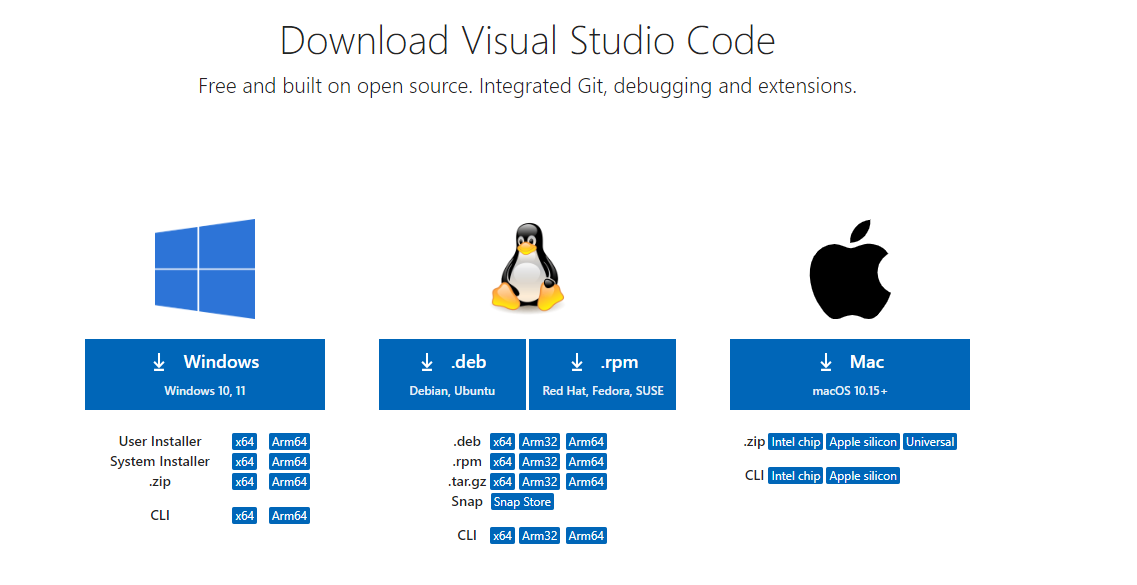
\includegraphics[width=12cm]{ESP32/VSCode//VSCode1}
            \caption{Visual Studio Code Download Links} 
        \end{figure}
    \end{itemize}
    
    
    
    \item After installation completes, launch VScode and choose "New File" to initiate the creation of a new file for testing purposes.
    \begin{figure}[H]
        \centering
        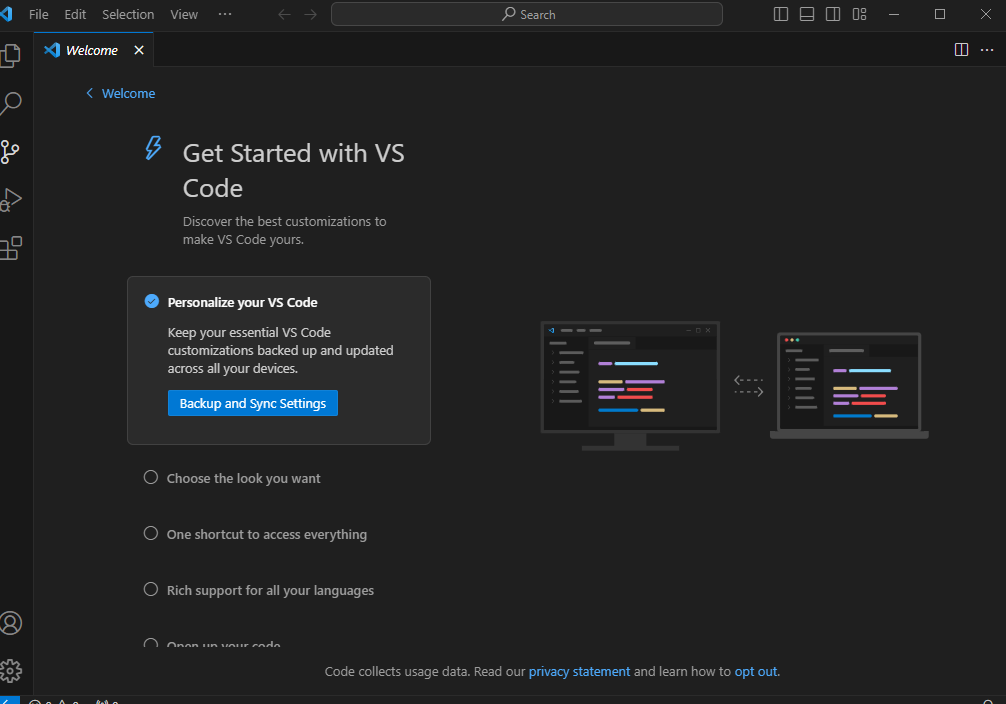
\includegraphics[width=12cm]{ESP32/VSCode//VSCode8}
        \caption{Visual Studio Code Window} 
    \end{figure}
    
    \item	For adding C/C++ extension,
    \begin{itemize}
        \item In Extensions tab, search for C/C++.
        \item Select Install.
        
        \begin{figure}[H]
            \centering
            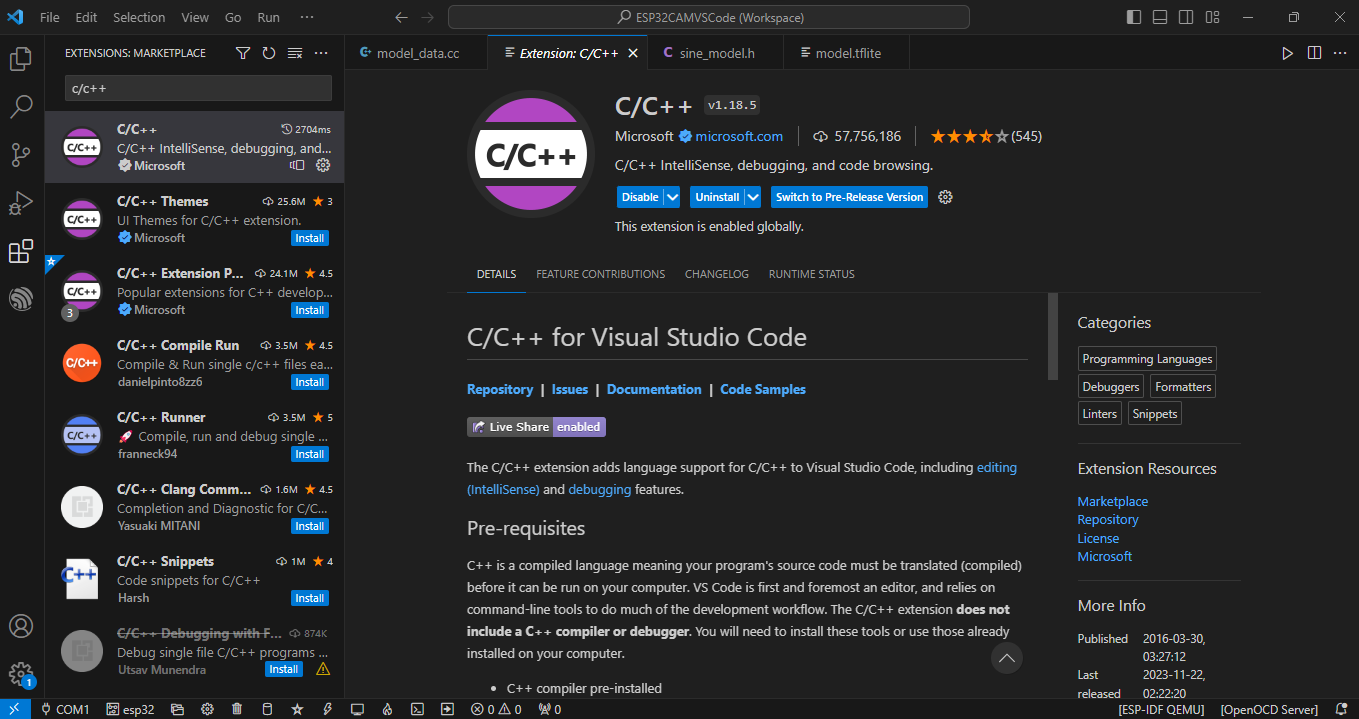
\includegraphics[width=12cm]{ESP32/VSCode//VSCode10}
            \caption{Visual Studio C/C++ Extension} 
        \end{figure}
    \end{itemize}
    
    
\end{enumerate}

\section{ESP-IDF Setup Process}

The ESP-IDF is an open-source software development framework developed by Espressif Systems. Specifically designed for their esp32 series of wifi and Bluetooth-enabled microcontrollers, the espidf provides a comprehensive set of tools, libraries, and documentation to facilitate the development of embedded applications. Below is the setup process:

\begin{enumerate}
    \item Open vscode.
    \begin{itemize}
        \item Open the Extensions.
        \item In the search bar, look for "esp-idf."
        \item Select the Install option for version 5.1.2.
        \begin{figure}[H]  
            \centering
            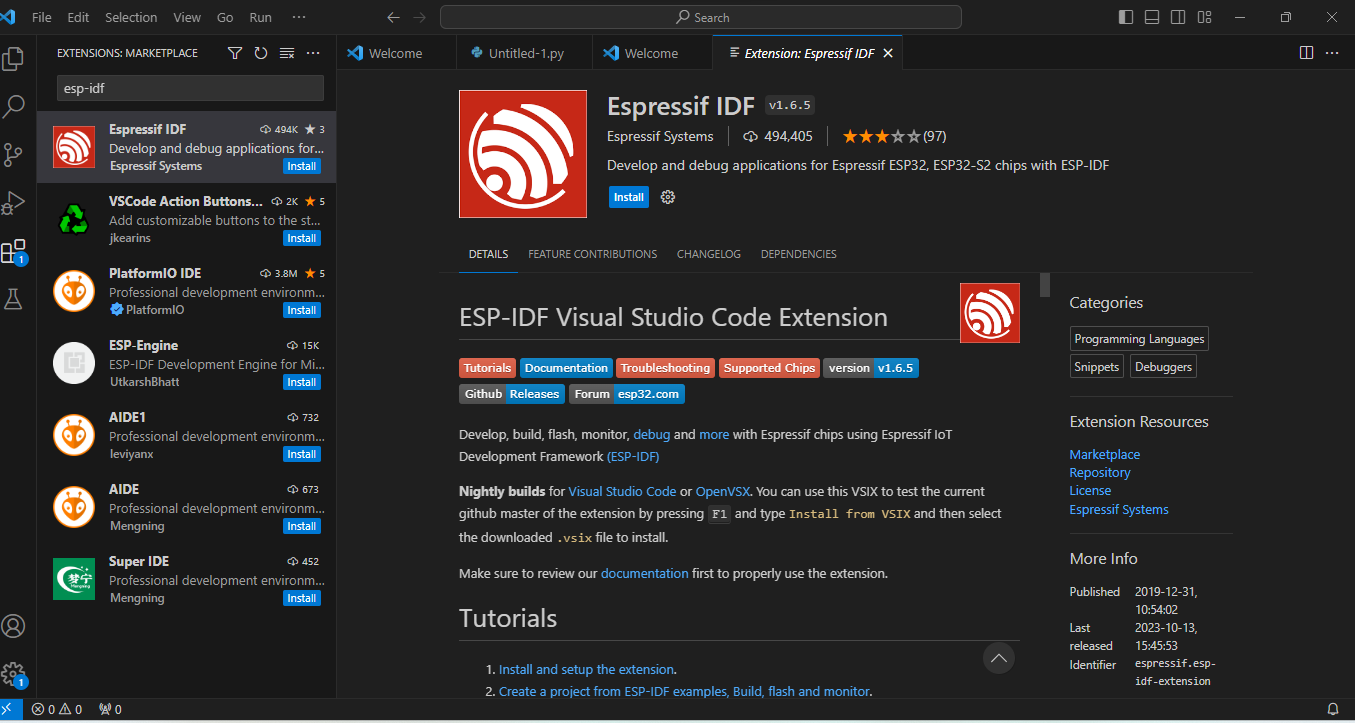
\includegraphics[width=12cm]{ESP32/ESPIDF/ESPIDF1}
            \caption{Visual Studio Code Installation "esp-df".} 
        \end{figure}
    \end{itemize}
    
    \item Select the ESP-IDF explorer.
    \begin{itemize}
        \item Choose "Express" from the options given.
        \item Select the Install option.
        \begin{figure}[H]   
            \centering
            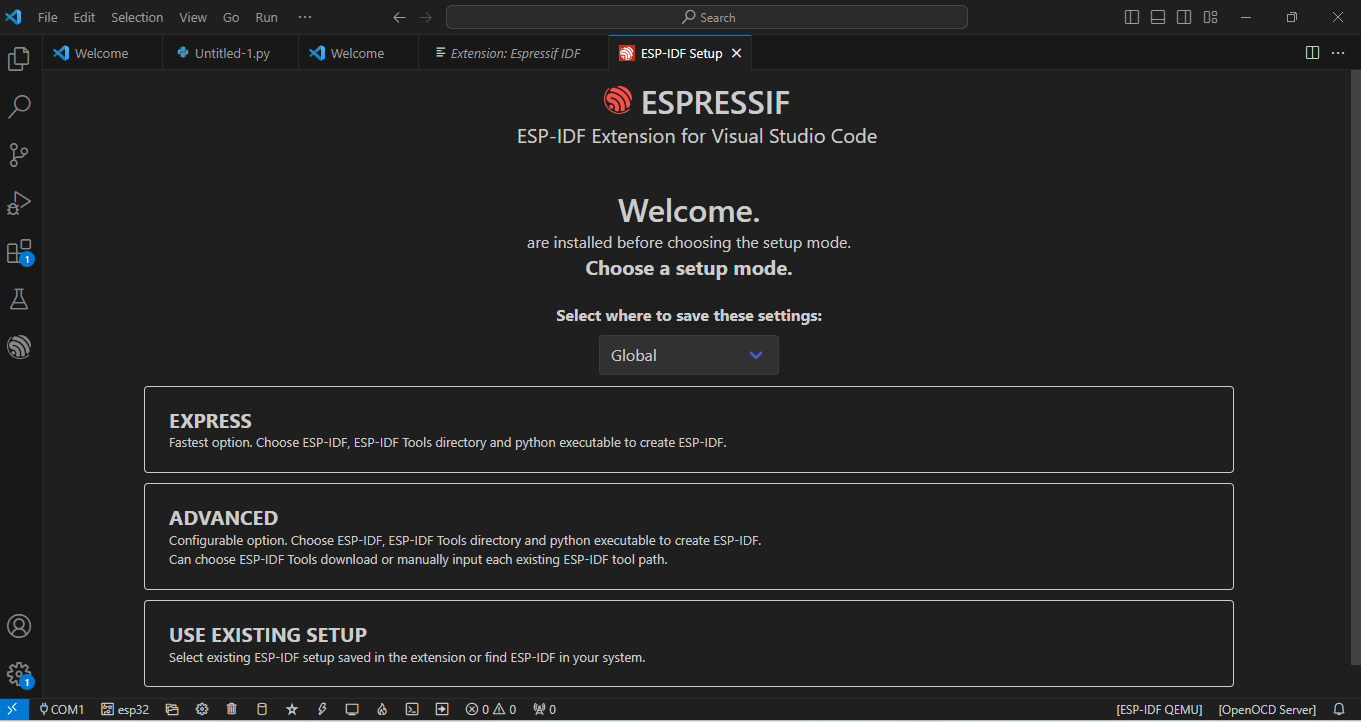
\includegraphics[width=12cm]{ESP32/ESPIDF/ESPIDF2}
            \caption{ ESP-IDF setup mode} 
        \end{figure}
    \end{itemize}
    
    \item Select Download Server: "Github."
    \begin{itemize}
        \item Select an ESP-IDF version to download (v5.1.2).
        \begin{figure}[H]] 
            \centering
            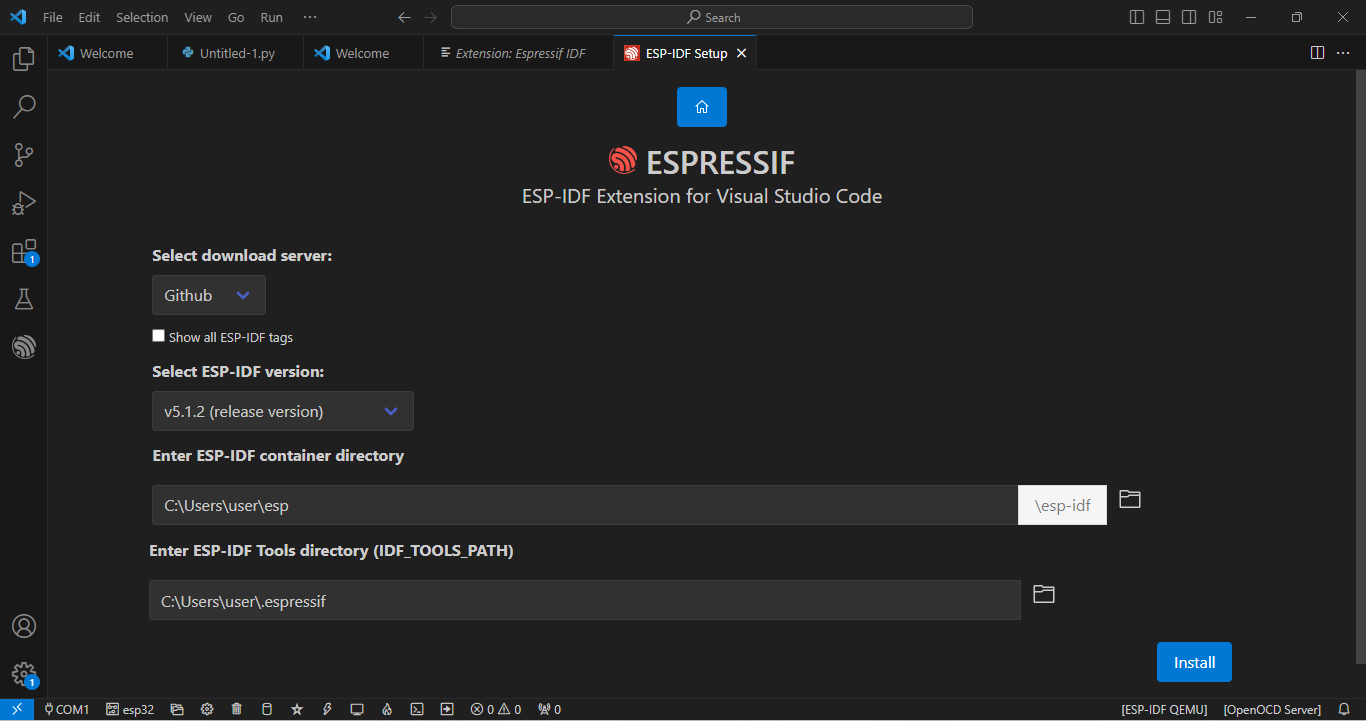
\includegraphics[width=12cm]{ESP32/ESPIDF/ESPIDF3}
            \caption{ ESP-IDF download server} 
        \end{figure}
    \end{itemize}
\end{enumerate}

Upon successful installation, a confirmation message will be displayed on the screen.
\begin{figure}[H]   
    \centering
    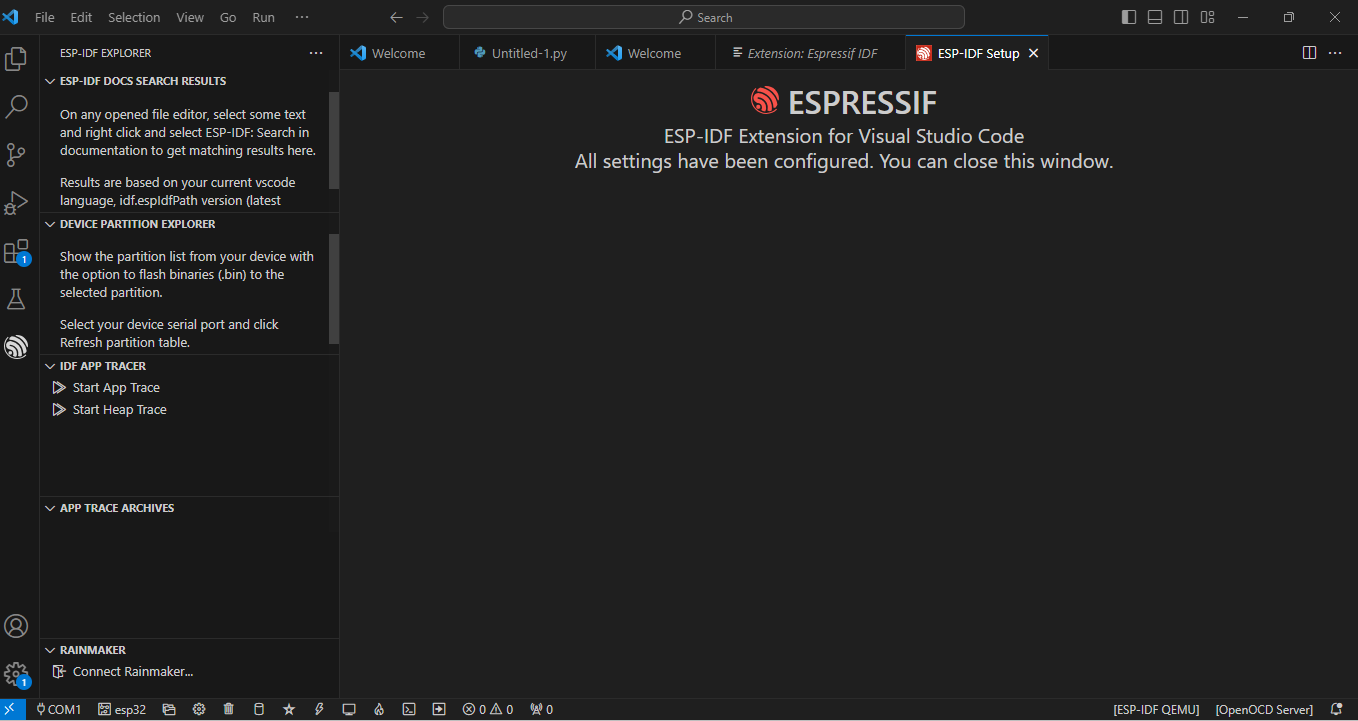
\includegraphics[width=12cm]{ESP32/ESPIDF/ESPIDF4}
    \caption{Successful installation of  ESP-IDF} 
\end{figure}


It is now time to install the esp32cam drivers. The first thing to do is to clone or download and extract the repository [ESP32 Camera GitHub project] to the components folder of your ESP-IDF. To do this, continue with the following steps:

\begin{enumerate}
    \item In your Directory Navigator, go to the "ESP-IDF" pre-installed folder and look for the "components" folder (i.e., "C:/Users/dereck/esp/esp-idf/components").
    
    \item Open Windows PowerShell.
    
    \item Run the following command to clone the ESP32 Camera GitHub project:
    
    \href{https://github.com/espressif/esp32-camera}{[ESP32 Camera GitHub project]}.
    
    
\end{enumerate}


\begin{figure}[H]   
    \centering
    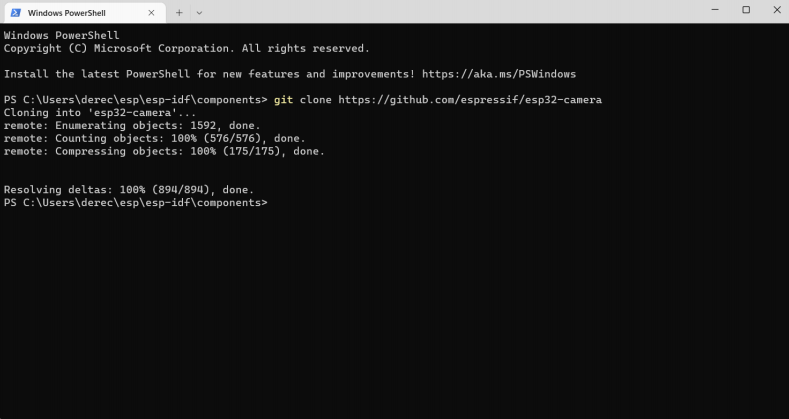
\includegraphics[width=12cm]{ESP32/ESP32clone}
    \caption{ESP32 Camera Clone Repository} 
\end{figure}

This will download and extract the necessary files for the esp32cam drivers into the designated components folder.




\begin{figure}
	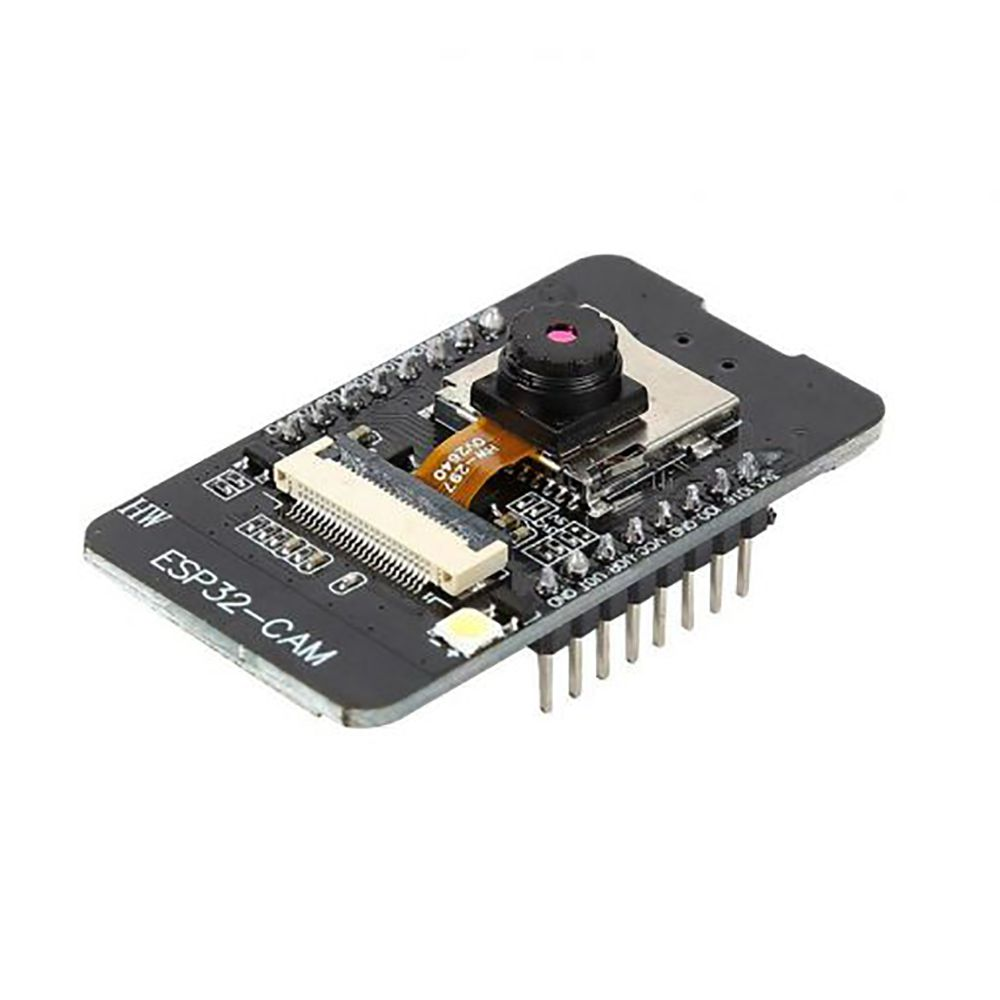
\includegraphics[width=\linewidth]{Esp32/ListMaterialESP32CAM}
	\caption{Esp32}
	\label{fig:arduino}
\end{figure}






